% Chapter 3
\chapter{Learning from Evolving Streams via Self-Training Windowing Ensembles (LESS-TWE)\label{chapter:contributions}}% For referencing the chapter elsewhere, use \ref{chapter:contributions} } % Main chapter title

In this chapter, we introduce our methodology, entitled Learning from Evolving Streams via Self-Training Novel Windowing Ensembles (LESS-TWE). First, we provide the reader with an overview of our framework, then discuss our contributions. These include a weighted soft voting scheme, a novel windowing technique that combines sliding and tumbling techniques, a non-selective self-training method, and the extension of an existing concept drift algorithm to remove its dependency on labelled data. Finally, we use a toy example to explain how data is processed from a stream.

\section{Overview of LESS-TWE}
Figure \ref{fig:prequential_loop} illustrates how our contributions fit together and operate in one iteration of an interleaved test-then-train loop (defined in section \ref{section:prequential}).

When predicting labels, data can arrive in chunks or one-by-one. In this example, data arrives one instance at a time. The first step is for the ensemble to predict a label for the new data instance; the classifiers in the ensemble each predict a label and a weighted soft vote scheme selects a winning label for the ensemble. The prediction confidence for that label is used to detect drifts. If a drift is detected, a subset of classifiers in the ensemble are first reset, and subsequently trained on a sliding window of previously seen labelled data (stored in the backup window). If no drifts were detected, then the label predicted replaces the real label value in the novel window, thereby self-training. This window stores $N$ times the number of instances processed at a time (in this example, one), where $N$ is the number of classifiers in the ensemble. A single classifier is trained per iteration of the interleaved test-then-train loop, in a cyclical manner, meaning that each classifier in the ensemble is trained only once every $N$ loop iterations. That is, a different classifier from the ensemble is trained at the next loop iteration.

Next, we provide a summary of our contributions.

\begin{sidewaysfigure}
  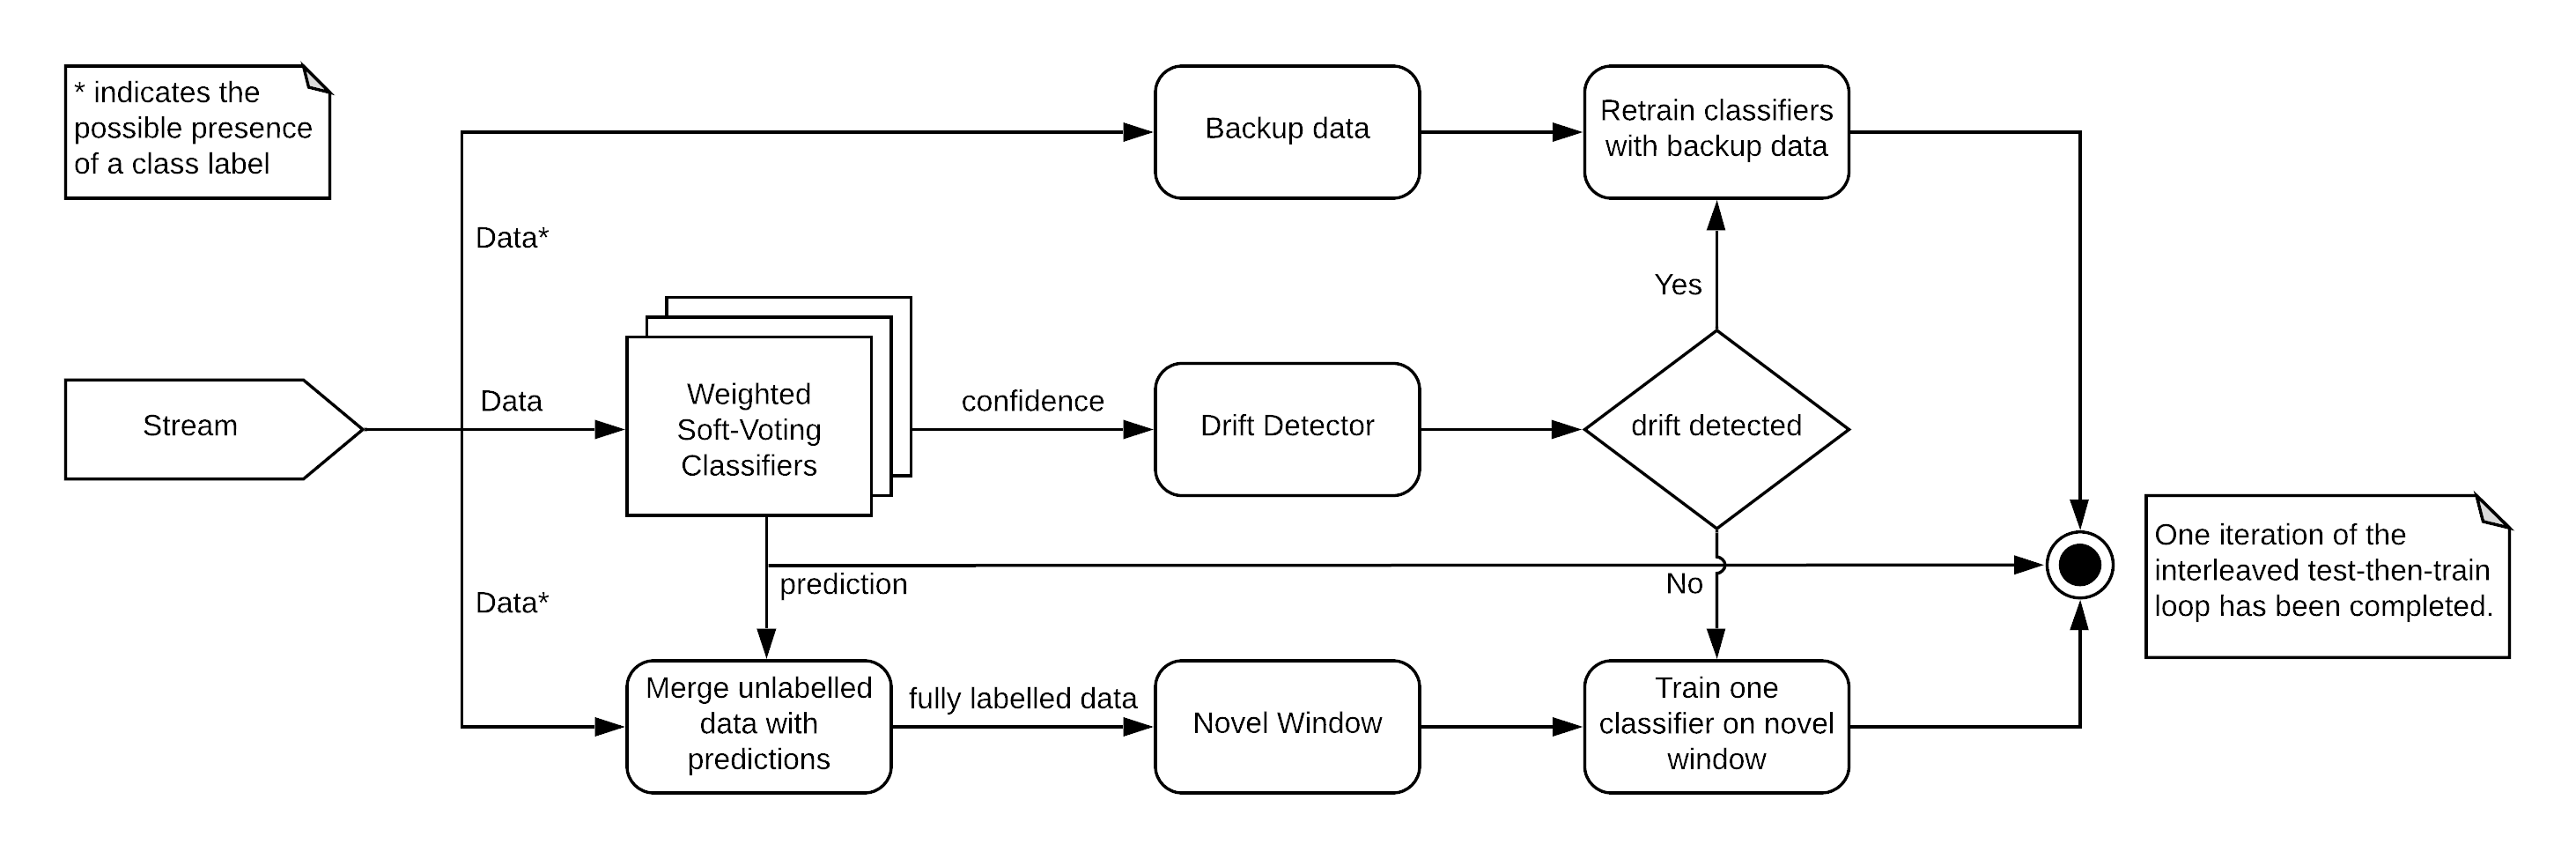
\includegraphics[width=\linewidth]{./images/chapter3/prequential_loop}
\caption{\label{fig:prequential_loop}High-Level Overview of the LESS-TWE methodology}
\end{sidewaysfigure}

\subsection{Summary of Contributions}

We propose a weighted soft voting scheme that uses a hyperbolic tangent function. We choose the \textit{tanh} function, as it allows us to approximate a logistic function while also being less computationally expensive \citep[10]{lecun2012efficient}.

Next, we propose a novel windowing technique, exclusive to ensembles. Our technique allows every classifier in the ensemble to train from each data point in the stream \textbf{exactly once} similar to tumbling windows, as opposed to sliding windows where a data point is trained on \textbf{at least once}. As such, our method presents a trade-off between accuracy and execution time. Only one classifier per batch is trained on the window, therefore each classifier trains on a specific data instance at different times, resulting in delayed training. This means that only one classifier in the ensemble is trained on the newest data before the ensemble predicts labels for the subsequent batch.
The motivation for this technique is to determine if we can spend less execution time training the classifiers and to investigate how progressively delaying training of some of the classifiers in the ensemble affects concept drift detection and classification performance.

Our next contribution relates to selective self-training. In this semi-supervised learning algorithm, a classifier assigns a label it predicts to unlabelled data for future learning, if it is highly confident it is correct. There have not yet been any attempts, to the best of our knowledge, to investigate how self-training performs if labelling all unlabelled data, regardless of the classifier's confidence in its predicted label.

Finally, our last contribution is an extension of the Fast Hoeffding Drift Detecting Method for evolving data Streams (FHDDMS), which detects drifts using the prequential accuracy. In our extension, we propose three schemes, one of which makes use of the average of the ensemble's classifiers' confidences. Our extension allows FHDDMS to run without any labelled data, therefore making it an unsupervised drift detector.

%----------------------------------------------------------------------------------------

\section{Voting Classifier: Weighting and Voting Schemes \label{section:new_voting_strategy}}

The reader may refer to section \ref{section:ensembles} for background on ensembles and voting classifiers.

A voting classifier was utilised from the mlxtend library\footnote{\url{http://rasbt.github.io/mlxtend/user_guide/classifier/EnsembleVoteClassifier/}}, developed by Sebastian Raschka. Mlxtend is an extension of the scikit-learn python machine learning library, to handle classification in a streaming setting.

The mlxtend voting classifier implements two voting strategies: the first being "soft" voting and the second being "hard" (majority) voting; refer to section \ref{section:voting_ensemble} for their definitions.

We implemented two additional soft voting schemes. These schemes require its classifiers to output a probability or confidence in the class label prediction. The first method makes use of a logistic function with a sigmoid curve to weight the probability, centred around a  confidence level. Let $\alpha$ be the parameter that defines the confidence level, let $\alpha=50\%$. The second method, explained soon thereafter is equivalent to the function of the first method while being less computationally intensive.


Logistic functions are defined by the function in equation \ref{eq:logistic_function}
\begin{equation}
    f(x)=\frac{L}{1+e^{-k(x-x_0)}}\\ 
    \label{eq:logistic_function}
\end{equation}
where \textit{e} is the natural logarithm base, \textit{$x_0$} is the x-value of the sigmoid's midpoint, \textit{L} is the curve's maximum value, and \textit{k} is the steepness of the curve.

The logistic function that we initially selected had the following values for the variables listed above: $x_0=0.65$, $L=1$, and $k=14$. These values were selected based on the resulting graph for values of $x \in [0, 1]$ and $f(x) \in [0, 1]$. As figure \ref{graph:weights} illustrates, predictions with less than approximately forty percent probability are essentially treated as predictions with zero probability; predictions with under a seventy percent probability are diminished in importance, and those over seventy percent are boosted. Refer to table \ref{table:weight_probabilities} to see how the values change by five and ten percent increments. The reasoning motivating this choice is our intuition that we should put more trust in predictions with over seventy percent (70\%) probability, put less trust in predictions with a probability of under seventy percent  (70\%), and virtually none in predictions with a probability of under forty percent (40\%).

\begin{figure}
  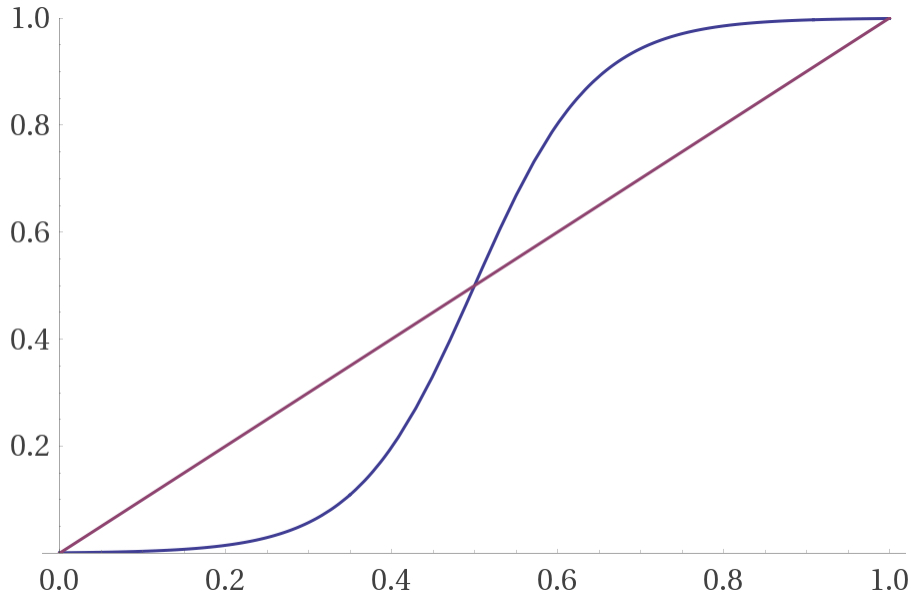
\includegraphics[width=\linewidth]{./images/chapter3/weight_graph}
\caption{\label{graph:weights}Voting classifier weighting functions\\\protect\blueline$x$\\
\protect\redline $\frac{1-tanh(3.5-7x)}{2}$}
\end{figure}

However, after extensive experimentation, of which the results are found in tables \ref{table:weighting_experimental_test} and \ref{table:weighting_experimental_test_all_datasets}, we found that setting \textbf{$x_0=0.50$} and \textbf{$k=14$} was more optimal than the values we initially selected through intuition for the $x_0$ and $k$ parameters.

The same test as above was repeated, but, over four separate data sets (SEA, SINE1, CIRCLES, MIXED which are covered in section \ref{section:datasets}) for the two best combinations of parameters and the one from our intuition ($k=14$, and $x_0 \in [0.5, 0.55, 0.65]$), and ran only once. Table \ref{table:weighting_experimental_test_all_datasets} shows, again, that $k=14, x_0=0.50$ seems to be the optimal set of parameters as it obtains the best results for three out of four data sets.

\begin{table}[]
\caption{\label{table:weighting_experimental_test}Experimental test of weighting function parameters}
\centering
\begin{tabular}{|c|c|c|c|c|}
\hline
\textbf{Parameters} & \textbf{Accuracy} & \textbf{$\kappa$} & \textbf{$\kappa_t$} & \textbf{$\kappa_m$} \\ \hhline{=====}
\textit{no weighting}&81.95&61.47&61.10&52.78 \\ \hline
10, 0.65&83.56&64.77&64.57&57.00 \\ \hline
14, 0.45&84.28&66.26&66.12&58.88 \\ \hline
\textbf{14, 0.50}&\textbf{84.77}&\textbf{67.34}&\textbf{67.17}&\textbf{60.15} \\ \hline
\textbf{14, 0.55}&\textbf{84.72}&\textbf{67.25}&\textbf{67.06}&\textbf{60.02} \\ \hline
14, 0.65&83.75&65.12&64.98&57.49 \\ \hline
14, 0.6&84.22&66.13&65.98&58.71 \\ \hline
14, 0.75&81.73&60.86&60.63&52.21 \\ \hline
14, 0.85&80.51&58.65&57.99&49.01 \\ \hline
5, 0.65&82.77&63.03&62.85&54.91 \\ \hline
7, 0.65&83.04&63.56&63.44&55.62 \\ \hline
\end{tabular}
\end{table}

\begin{table}
\caption{\label{table:weighting_experimental_test_all_datasets}Experimental test of weighting function parameters on 4 datasets}
\centering
\begin{tabular}{|c|c|c|c|c|c|}
\hline
\textbf{Dataset} & \textbf{Parameters} ($k=14$) & \textbf{Accuracy} & \textbf{$\kappa$} & \textbf{$\kappa_t$} & \textbf{$\kappa_m$} \\ \hhline{======}
& $x_0=0.5$    &    84.30    &    68.60    &    68.69    &    68.73\\ \cline{2-6}
sine1 & $x_0=0.55$    &    84.15    &    68.30    &    68.39    &    68.44\\ \cline{2-6}
 & $x_0=0.65$    &    83.79    &    67.59    &    67.67    &    67.72\\ \hhline{======}
 & $x_0=0.5$    &    79.95    &    59.90    &    60.07    &    60.12\\ \cline{2-6}
mixed & $x_0=0.55$    &    79.89    &    59.78    &    59.96    &    60.01\\ \cline{2-6}
 & $x_0=0.65$    &    79.60    &    59.20    &    59.38    &    59.43\\ \hhline{======}
 & $x_0=0.55$    &    79.72    &    59.45    &    59.44    &    59.15\\ \cline{2-6}
circles & $x_0=0.65$    &    79.43    &    58.87    &    58.87    &    58.57\\ \cline{2-6}
 & $x_0=0.5$    &    77.72    &    55.45    &    55.45    &    55.13\\ \hhline{======}
 & $x_0=0.5$    &    85.20    &    68.27    &    68.10    &    61.28\\ \cline{2-6}
SEA & $x_0=0.55$    &    84.25    &    66.25    &    66.05    &    58.80\\ \cline{2-6}
 & $x_0=0.65$    &    83.41    &    64.38    &    64.25    &    56.60\\ \hline
\end{tabular}
\end{table}

\begin{table}[]
\caption{\label{table:weight_probabilities}Probabilities after weighting}
\centering
\begin{tabular}{|c|c|c|c|c|c|c|c|c|c|c|c|} \hline
\textbf{Probability (\%)} & 0-10&20&30&40&50&60&65&70&75&80-85&90-100 \\ \hline
\textbf{Weighted (\%)} & 0&1&6&20&50&80&89&94&97&99&100 \\ \hline
\end{tabular}
\end{table}

We must note that $\forall x \in [0,1], f(x) \in [0, \frac{1}{1+e^{-7}}\approx 0.9991]$ for the function in equation \ref{eq:logistic_function} , we could then divide the function by its value for the maximum value for $p_i(X)$ (which is 1) to ensure that our function covers all values in $[0,1]$, but this is unnecessary as all values will be be in the same range, and it adds another calculation.
Refer to figure \ref{graph:weights} for the plot of equation \ref{eq:logistic_function_params}.

\begin{equation}
\frac{1}{1+e^{-14(p_i(X)-0.50)}}
\label{eq:logistic_function_params}
\end{equation}

Our proposed voting strategy therefore computes the average of this logistic function using the prediction of each classifier for each class label. See the following equation:
\begin{equation}
\frac{1}{n}\sum_{i=1}^{n}\frac{1}{1+e^{-14(p_i(X)-0.50)}}\\ 
    \label{eq:logistic_sum}
\end{equation}
where $n$ is the number of classifiers in the voting ensemble, and $p_i(X)$ is the probability of classifier $i$ predicting that the tuple in question belongs to class X.

We propose another weighting equation to determine if it is possible to achieve similar results by using a different function that resembles the logistic sigmoid function presented above while being less computationally intensive. As LeCun states in \citep[10]{lecun2012efficient},  "hyperbolic tangent functions often converge faster than the standard logistic function".
Our hyperbolic tangent weighting function is seen in equation \ref{eq:tanh_weight_fn} and the sum is seen in equation \ref{eq:tanh_sum}. The plot of equation \ref{eq:tanh_weight_fn} is completely identical to the plot of equation \ref{eq:logistic_function}.
\begin{equation}
    f(x)=\frac{1-tanh(3.5-7x)}{2}
    \label{eq:tanh_weight_fn}
\end{equation}
\begin{equation}
\frac{1}{n}\sum_{i=1}^{n} \frac{1-tanh(3.5-7\times p_i(X))}{2}
    \label{eq:tanh_sum}
\end{equation}
The calculation of averages presented in equations \ref{eq:logistic_sum} and \ref{eq:tanh_sum} are calculated for each class label. The class label with the highest average is thereafter selected as the winner in the vote. We aim to test the hypothesis that weighting the predictions by an exaggeration of their probability will increase the accuracy of our voting classifier.

In order to confirm that the new weighting function was more computationally efficient, we compared the total running time to evaluate each weighting function ten million times on a random value in [0, 1]. The benchmark showed, as seen in table \ref{table:weight_benchmark}, that the logistic function takes almost 3.5 times longer to compute than the hyperbolic tangent function, which will, therefore, be used for the remainder of this thesis.

\begin{table}[]
\centering
\caption{\label{table:weight_benchmark}Weighting function benchmark results}
\begin{tabular}{|c|c|}
\hline
\textbf{Sigmoid function} & \textbf{Hyperbolic tangent} \\ \hhline{==}
1441.05 ns/class/loop & 407.40 ns/class/loop \\ \hline
\end{tabular}
\end{table}

Algorithm \ref{alg:new_voting_scheme} shows the implementation of this new voting scheme using the hyperbolic tangent function. Figure \ref{graph:weights} plots the proposed weighting function and an unweighted prediction represented by $f(x) =x$, for  $x \in [0,1]$. This figure shows how much a value is boosted or reduced compared to its original value.

Given that the hyperbolic tangent function selected is equivalent to the logistic sigmoid function, it is not necessary to test its parameters experimentally as they give the exact same output (difference between the two functions at any given point does not exceed much more than $10^{-16}$). Figure \ref{fig:boxplots_params} shows the boxplots of table \ref{table:weighting_experimental_test}. The whiskers correspond to the minimum and maximum values over 10 runs with each parameter. The dotted diamond corresponds to the standard deviation, the dotted line in the box corresponds to the mean, while the solid line corresponds to the median.

\begin{figure}
  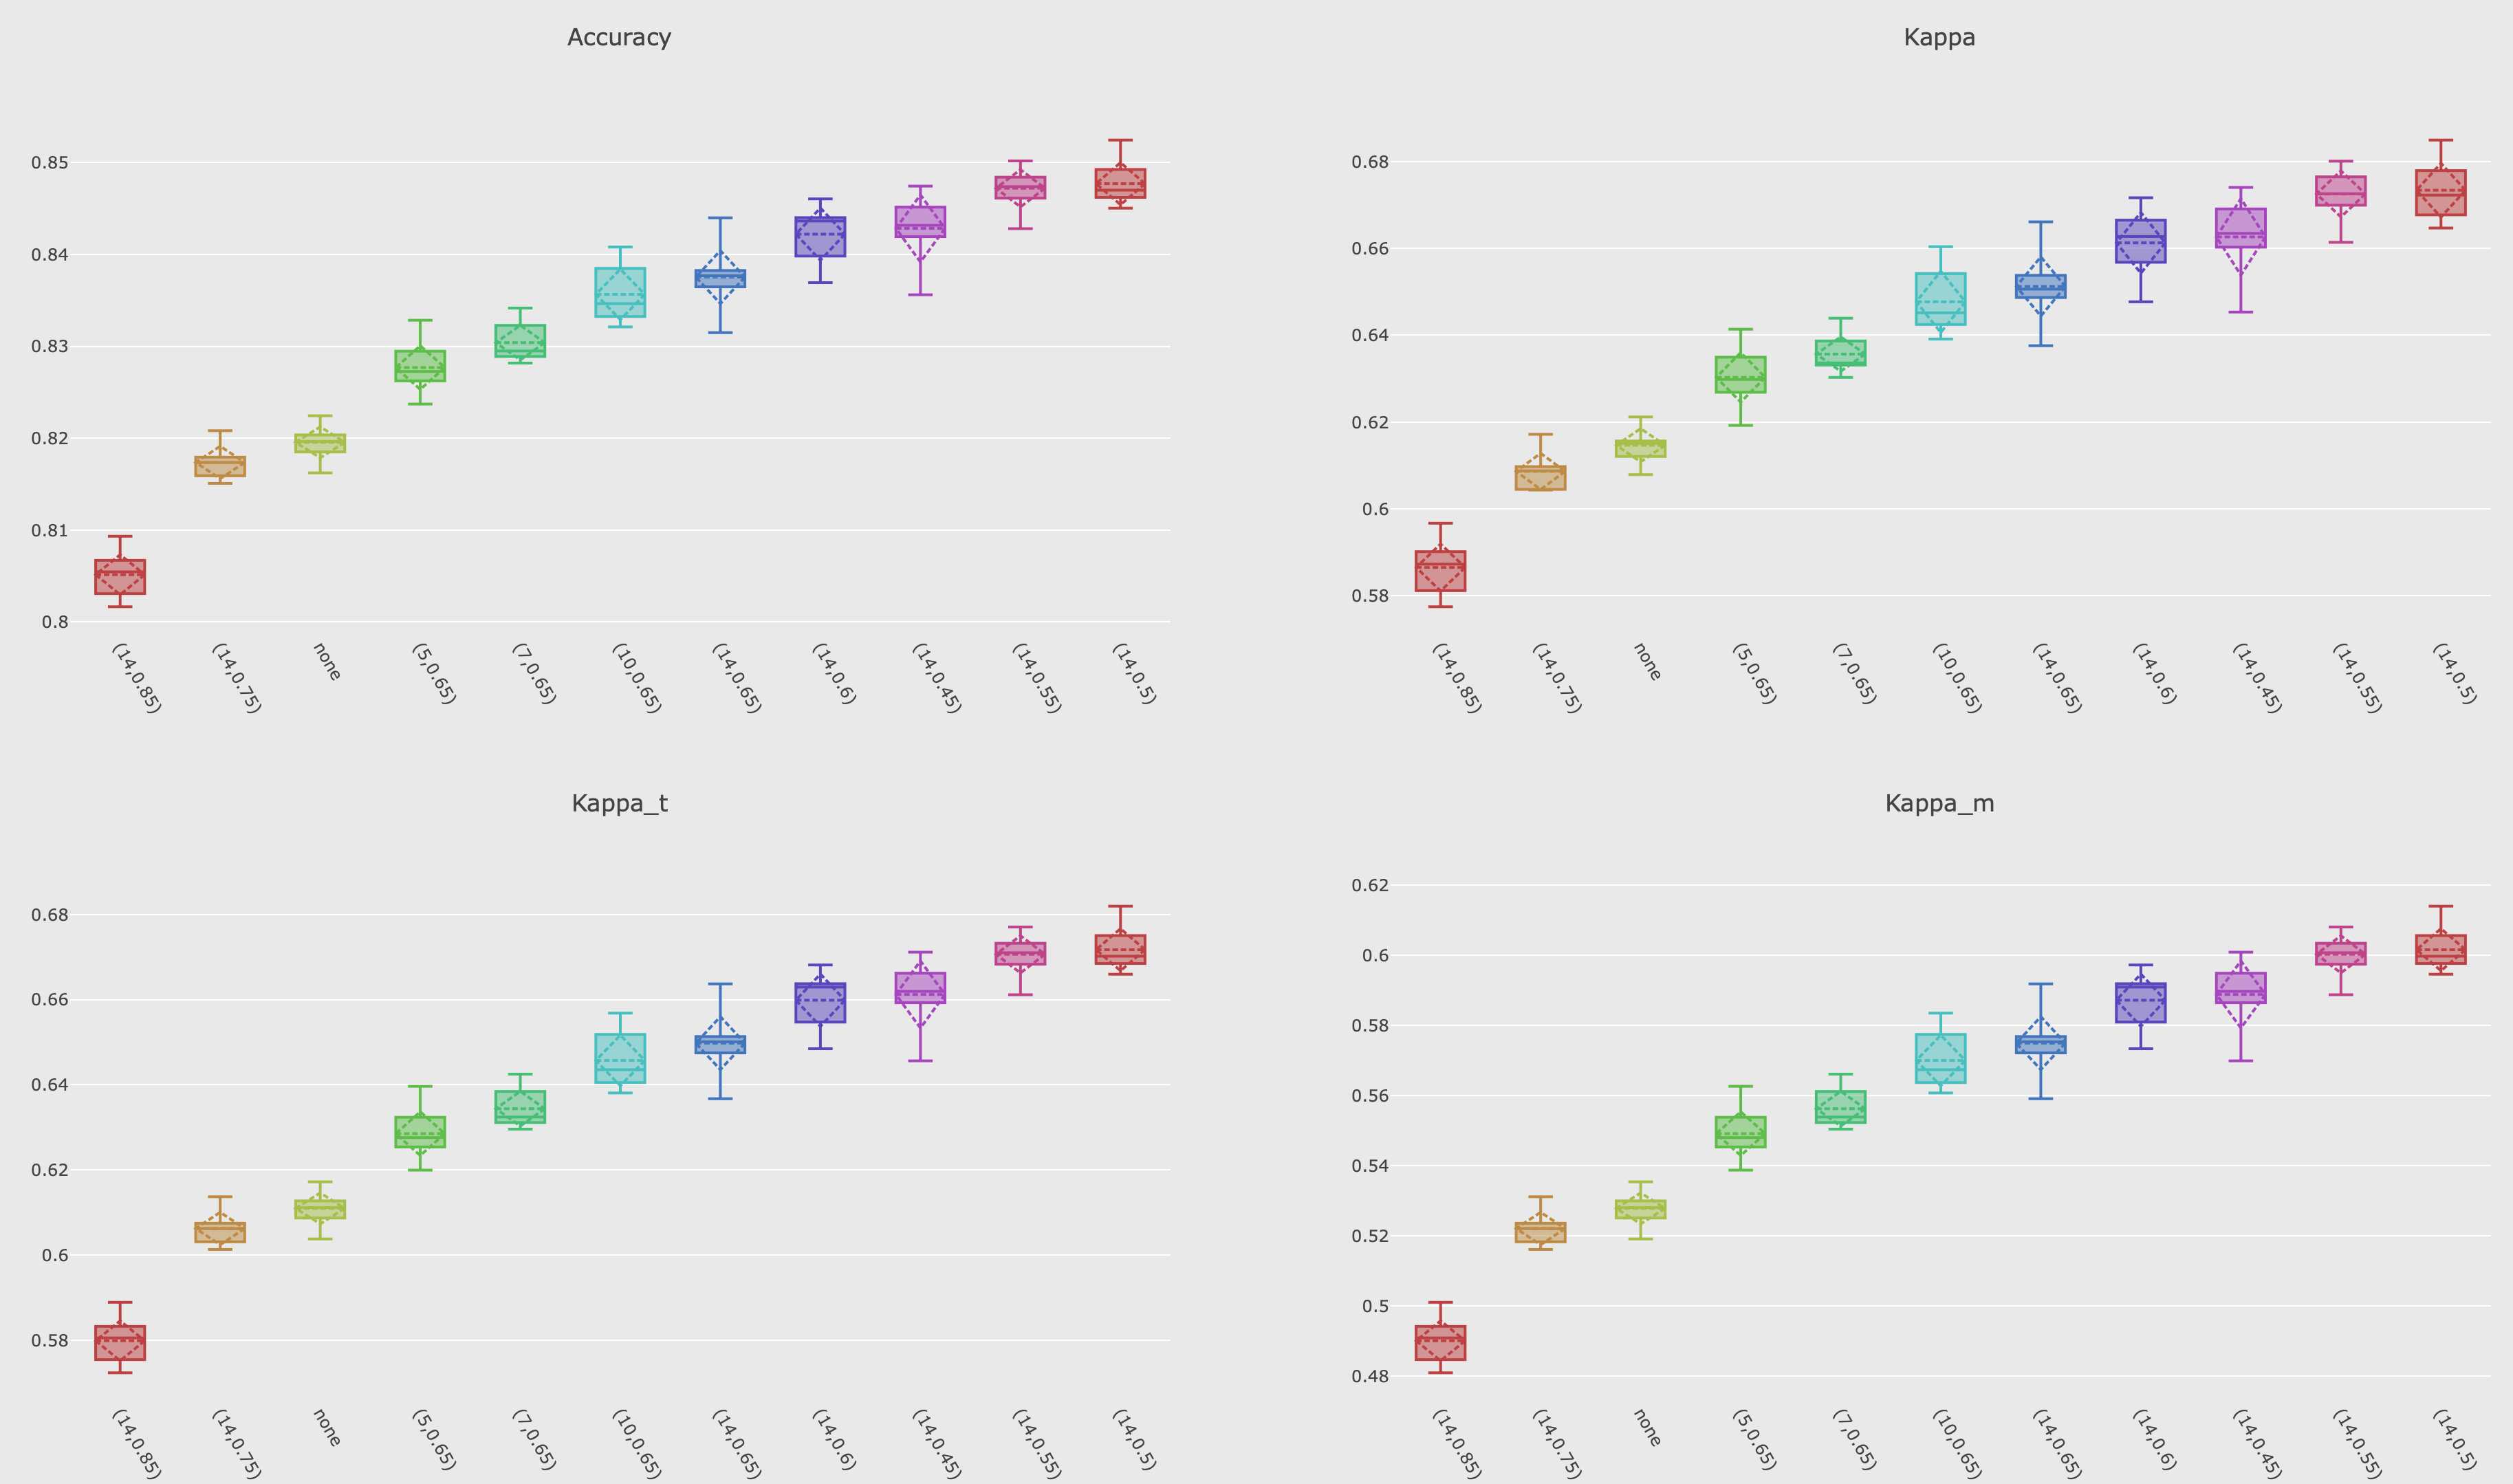
\includegraphics[width=\linewidth]{./images/chapter3/boxplots_params}
\caption{\label{fig:boxplots_params}Boxplots of experimental test for logistic function parameters}
\end{figure}


\begin{algorithm}
    \caption{\label{alg:new_voting_scheme}tanh weighting scheme for voting classifier}
    \Fn{voting\_classifier.predict(X)}{
        \tcc{The probabilities are stored in a $1\times2$ matrix (using binary classification for simplicity) where each column represents a class, and each row represents a sub-classifier}
        weighted\_probabilities = []\;
        \ForEach{$classifier \in voting.classifiers$}{
            array = classifier.predict()\;
            $w\_p$ = [weight(array[0]), weight(array[1])]\;
            weighted\_probabilities.append($w\_p$)\;
        }
        \tcp{map sub-classifier probabilities to single probability}
        avg = weighted\_probabilities.avg\_over\_columns()\;
        prediction, prediction\_probability = max(avg), class\_max\_value(avg)\;
        \Return{prediction, prediction\_probability}\;
    }
    \Fn{weight(p)}{
        \Return $\frac{1-tanh(3.5-7p)}{2}$\;
    }
\end{algorithm}



%----------------------------------------------------------------------------------------

\section{Hybrid sliding-tumbling windows\label{section:hybrid-windows}}
In \cite{KRAWCZYK2017132}, Krawczyk mentions that one of the many issues in data stream mining is execution time, in the sense that our algorithm must learn faster than tuples can arrive. In our case, we aim to determine if we can delay training of some classifiers in our ensemble, and how it affects execution time and classifying performance, as well as drift detection performance.

We propose the following algorithm, implemented in algorithm \ref{alg:sliding_tumbling_windows}, titled \textit{Sliding-Tumbling Windows for Training Ensembles}.
Let the number of tuples (single tuple or chunk) used in the interleaved test-then-train loop iterations be \textit{number\_of\_tuples}, and let \textit{number\_of\_classifiers} be the number of classifiers in the ensemble. The ensemble will have a window size of \textit{number\_of\_tuples} $\times$ \textit{number\_of\_classifiers}. At every iteration of the interleaved test-then-train loop, we will append the new tuples to the ensemble's window and train a single classifier in the ensemble on that window. For the next \textit{number\_of\_classifiers - 1} iterations, we will train the remaining \textit{number\_of\_classifiers - 1} classifiers in the ensemble. We do this so that from the point of view of the ensemble, we are training using sliding windows. However, from the point of each classifier in the ensemble, we are training them using tumbling windows.

While not used for the same purpose, the same sliding batches were used to improve CDC-Stream in \citep{d2016fine,d2017context}. Figure \ref{fig:sliding_tumbling_windows}, taken from D'Ettore's thesis, shows how the algorithm works for three (3) classifiers in the ensemble with a batch size of one (1) and a window size of three (3). Each classifier will only learn from the same coloured batch; meaning that at time \textit{t}, only a single classifier has enough tuples to learn from, but the others will learn at time \textit{t+1} and finally at time \textit{t+2}. Each classifier will be learning from what essentially is a tumbling window, from their point of view, just not all from the same one, or at the same time. 

To clarify the example, (using figure \ref{fig:sliding_tumbling_windows}) at time $t_1$, our ensemble will receive only one instance, add it to the sliding window and train classifier $c_1$ on the window. At time $t_2$, another instance will be added to the window and the ensemble will train classifier $c_2$ on the new window containing two tuples. At time $t_3$, the ensemble will train classifier $c_3$ on the first purple chunk (the window now has its maximum of 3 instances). At time $t_4$, $c_2$ will learn from the first blue chunk. And at time $t_5$, $c_3$ will learn from the first green chunk. This process loops indefinitely. 

The motivation for this technique is to determine if we can spend less execution time training the classifiers. We also aim to investigate how progressively delaying training of some of the classifiers in the ensemble affects concept drift detection and classification performance while also hopefully reducing execution time.

\begin{algorithm}
\KwResult{at least one classifier in the ensemble was trained}
\tcp{voting\_ensemble stores a classifier list, its count, and, the index of the current classifier to train}
\Fn{ensemble.train(X, y)}{    
        classifier\_to\_train = classifier\_list[index]\;
        index = (index + 1) modulo (number\_of\_classifiers)\;
        classifier\_to\_train.partial\_train(X, y)\;
}
\caption{Sliding-Tumbling Windows for Training Ensembles\label{alg:sliding_tumbling_windows}}
\end{algorithm}

\begin{figure}
  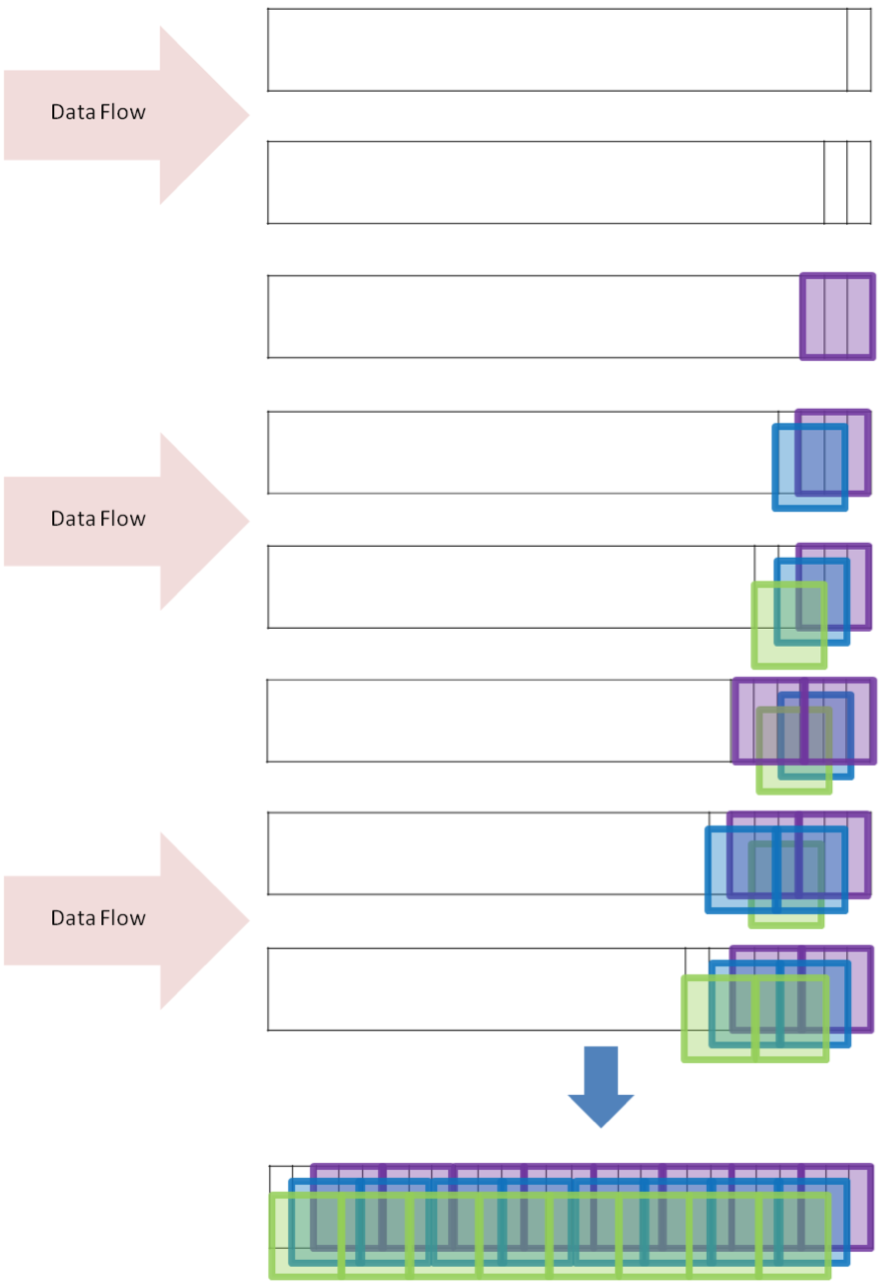
\includegraphics[width=\linewidth]{./images/chapter3/sliding_tumbling_windows}
  \caption{Sliding Tumbling windows \citep{d2016fine}.}
  \label{fig:sliding_tumbling_windows}
\end{figure}



%----------------------------------------------------------------------------------------

\section{Non-Selected Self-Training \label{section:vc_reduce_gt}}

The interleaved test-then-train methodology in a data streaming setting has a rather significant flaw if we consider a real-life scenario: we are assuming that we obtain the ground truth immediately after testing. This means that we assume that the ground truth is always available in a fraction of a second after testing our models. For the vast majority of cases, this approach is not realistic, again, in a real-world setting.

Therefore, we aim to determine if we could re-use the idea behind self-training in an offline setting to reduce our dependency on labelled data in the online streaming setting for the interleaved test-then-train method. We propose an approach that is, as previously stated, similar to selective self-training in that we use the classifier's prediction, as opposed to correctly labelled instances, when training.

However, using only the predictions to train our model in an online setting is a recipe for disaster. The known cons to using self-training in an offline setting are that it can reinforce classification errors; it is, therefore, logical for us to conclude that we will encounter the same risks in porting this idea to a streaming setting.

Given the restriction of limiting reinforcing misclassification errors, our goal is to determine at what ratio of predictions to ground-truth our voting ensemble's accuracy would decline and by how much.

The algorithm behind this idea is very straightforward: it consists in duplicating the class label array and replacing at random a given fraction of true labels with predictions from the ensemble, if a drift was not detected right before. See algorithm \ref{alg:self-training} for the pseudocode (function \textit{swap ground truth with predictions}).

\begin{algorithm}
\While{stream.has\_more\_instances()}{
    X, y = stream.get\_next\_tuples(number\_of\_instances\_to\_fetch)\;
    predictions, probabilities = voting\_ensemble.predict(X)\;
    drift\_detected = voting\_ensemble.detect\_drift(predictions, probabilities)\;
    \If{$percentage \neq 100$ \textbf{and} drift not detected}{
        y = swap\_ground\_truth\_with\_predictions(y, predictions, percentage)\;
    }
 voting\_ensemble.train(X, y)\;
}

\tcp{This algorithm only shows the steps required to modify the ground truth array}
\Fn{swap\_ground\_truth\_with\_predictions(y, predictions, percentage)}{
    \For{$index=0\ \textbf{;}\ index < length(y)\ \textbf{;}\ index += 1$}{
        \If{random\_number\_between(0, 100) > percentage}{
            y[index] = predictions[index]\;
        }
    }
    \Return{y}\;
}
\caption{\label{alg:self-training}Online self-training}
\end{algorithm}

%----------------------------------------------------------------------------------------

\section{Extending FHDDM/S to function without labelled data}

Additionally, this thesis builds upon Pesaranghader's work described in section \ref{section:fhddm/s}

FHDDMS, the drift detection algorithm proposed by Pesaranghader in \cite{pesaranghader2016fast} relies on the immediate knowledge of labelled data. The drift detection mechanism in FHDDMS relies on storing, in a sliding window, whether or not the classifier correctly predicted the class. This method only applies to a select few domains where the correct label becomes available almost instantaneously after the data arrives, and to all synthetic data streams of course. For the vast majority of domains, this method is not applicable.

It is for that reason that we have set out to study if FHDDM/S is still able to detect drifts when completely removing its dependency on any knowledge of the ground truth in an online streaming setting.

In order to do so, we have opted to extend FHDDM and FHDDMS such that its sliding window(s) now store(s) either a numerical value for a prediction probability, or a different boolean.

Our extension, if using prediction probabilities, requires classifiers that can output such values. When predicting the class for a data point, each classifier in the ensemble outputs its probability for each class label. For example, a classifier could output the following class probabilities for a non-binary classification task $\{A: 24\%, B: 11\%, C: 65\%\}$.

We implemented three approaches. The first two use multiple drift detectors, one per classifier in the ensemble. In addition, the third uses a single drift detector by averaging values from each classifier. The drift detector in question is our extended version of FHDDM/S.

The first approach stores boolean values in its detectors' sliding windows. The boolean value indicates if a classifier predicted the class that was voted as the winner for the ensemble.

In the second, each window stores its classifier's probability for the class that won the vote. These values may or may not be weighted, using the hyperbolic tangent function from section \ref{section:new_voting_strategy}.

The last method also stores class probabilities, but stores the \textit{average} probability from all classifiers in the ensemble into a single window in a single drift detector. As for the previous approach, the probabilities that averaged are those for the winning class. Furthermore, the values may or may not be weighted using that same function, as for the previous approach.

After extensive experimentation, results indicate that the unweighted probabilities were no more useful than the weighted values for detecting drifts as the difference in performance between the two is negligible. \textbf{To illustrate, a} SEA dataset was generated with 10\% noise with one-hundred thousand instances, with four concepts and three abrupt concept drifts at every twenty-five thousand instances. The $CIRCLES$, $MIXED$ and $SINE1$ datasets were also used (refer to section \ref{section:performance_measures}). When drifts are detected, all of the classifiers in the ensemble were completely reset, and one drift detector for the entire ensemble was used. In order to determine whether to use unweighted or weighted probabilities for the drift detector, we looked at the accuracy and kappa statistics of the entire stream (covered in section \ref{eq:kappa}). Table \ref{table:drift_use_weighting_experimental_test} shows these results. The values in the table are averages over ten runs.

\begin{table}[]
\caption{\label{table:drift_use_weighting_experimental_test}Testing whether to use weighted probabilities for detecting drifts}
\centering
\begin{tabular}{|c|c|c|c|c|c|}
\hline
\textbf{Dataset} & \textbf{Weighted/Unweighted} & \textbf{Accuracy} & \textbf{$\kappa$} & \textbf{$\kappa_t$} & \textbf{$\kappa_m$} \\ \hhline{======}
SEA&\checkmark&84.53&66.77&66.66&59.53\\ \cline{2-6}
 &$\times$&84.42&66.51&66.42&59.23\\ \hhline{======}
circles&$\times$&78.35&56.71&56.70&56.39\\ \cline{2-6}
 &\checkmark&78.25&56.51&56.50&56.19\\ \hhline{======}
mixed&\checkmark&80.00&60.00&60.18&60.23\\ \cline{2-6}
 &$\times$&79.97&59.94&60.11&60.16\\ \hhline{======}
sine1&\checkmark&84.35&68.71&68.79&68.84\\ \cline{2-6}
 &$\times$&84.30&68.60&68.68&68.73\\ \hline
\end{tabular}
\end{table}

Figure \ref{fig:boxplot_params_use_w} illustrates the results of experimentation in table \ref{table:drift_use_weighting_experimental_test} through the use of boxplots. The weighted predictions cause performance to increase ever so slightly. However, in the case of the $CIRCLES$ dataset, the unweighted probabilities seem to perform better than the weighted ones.

\begin{figure}
  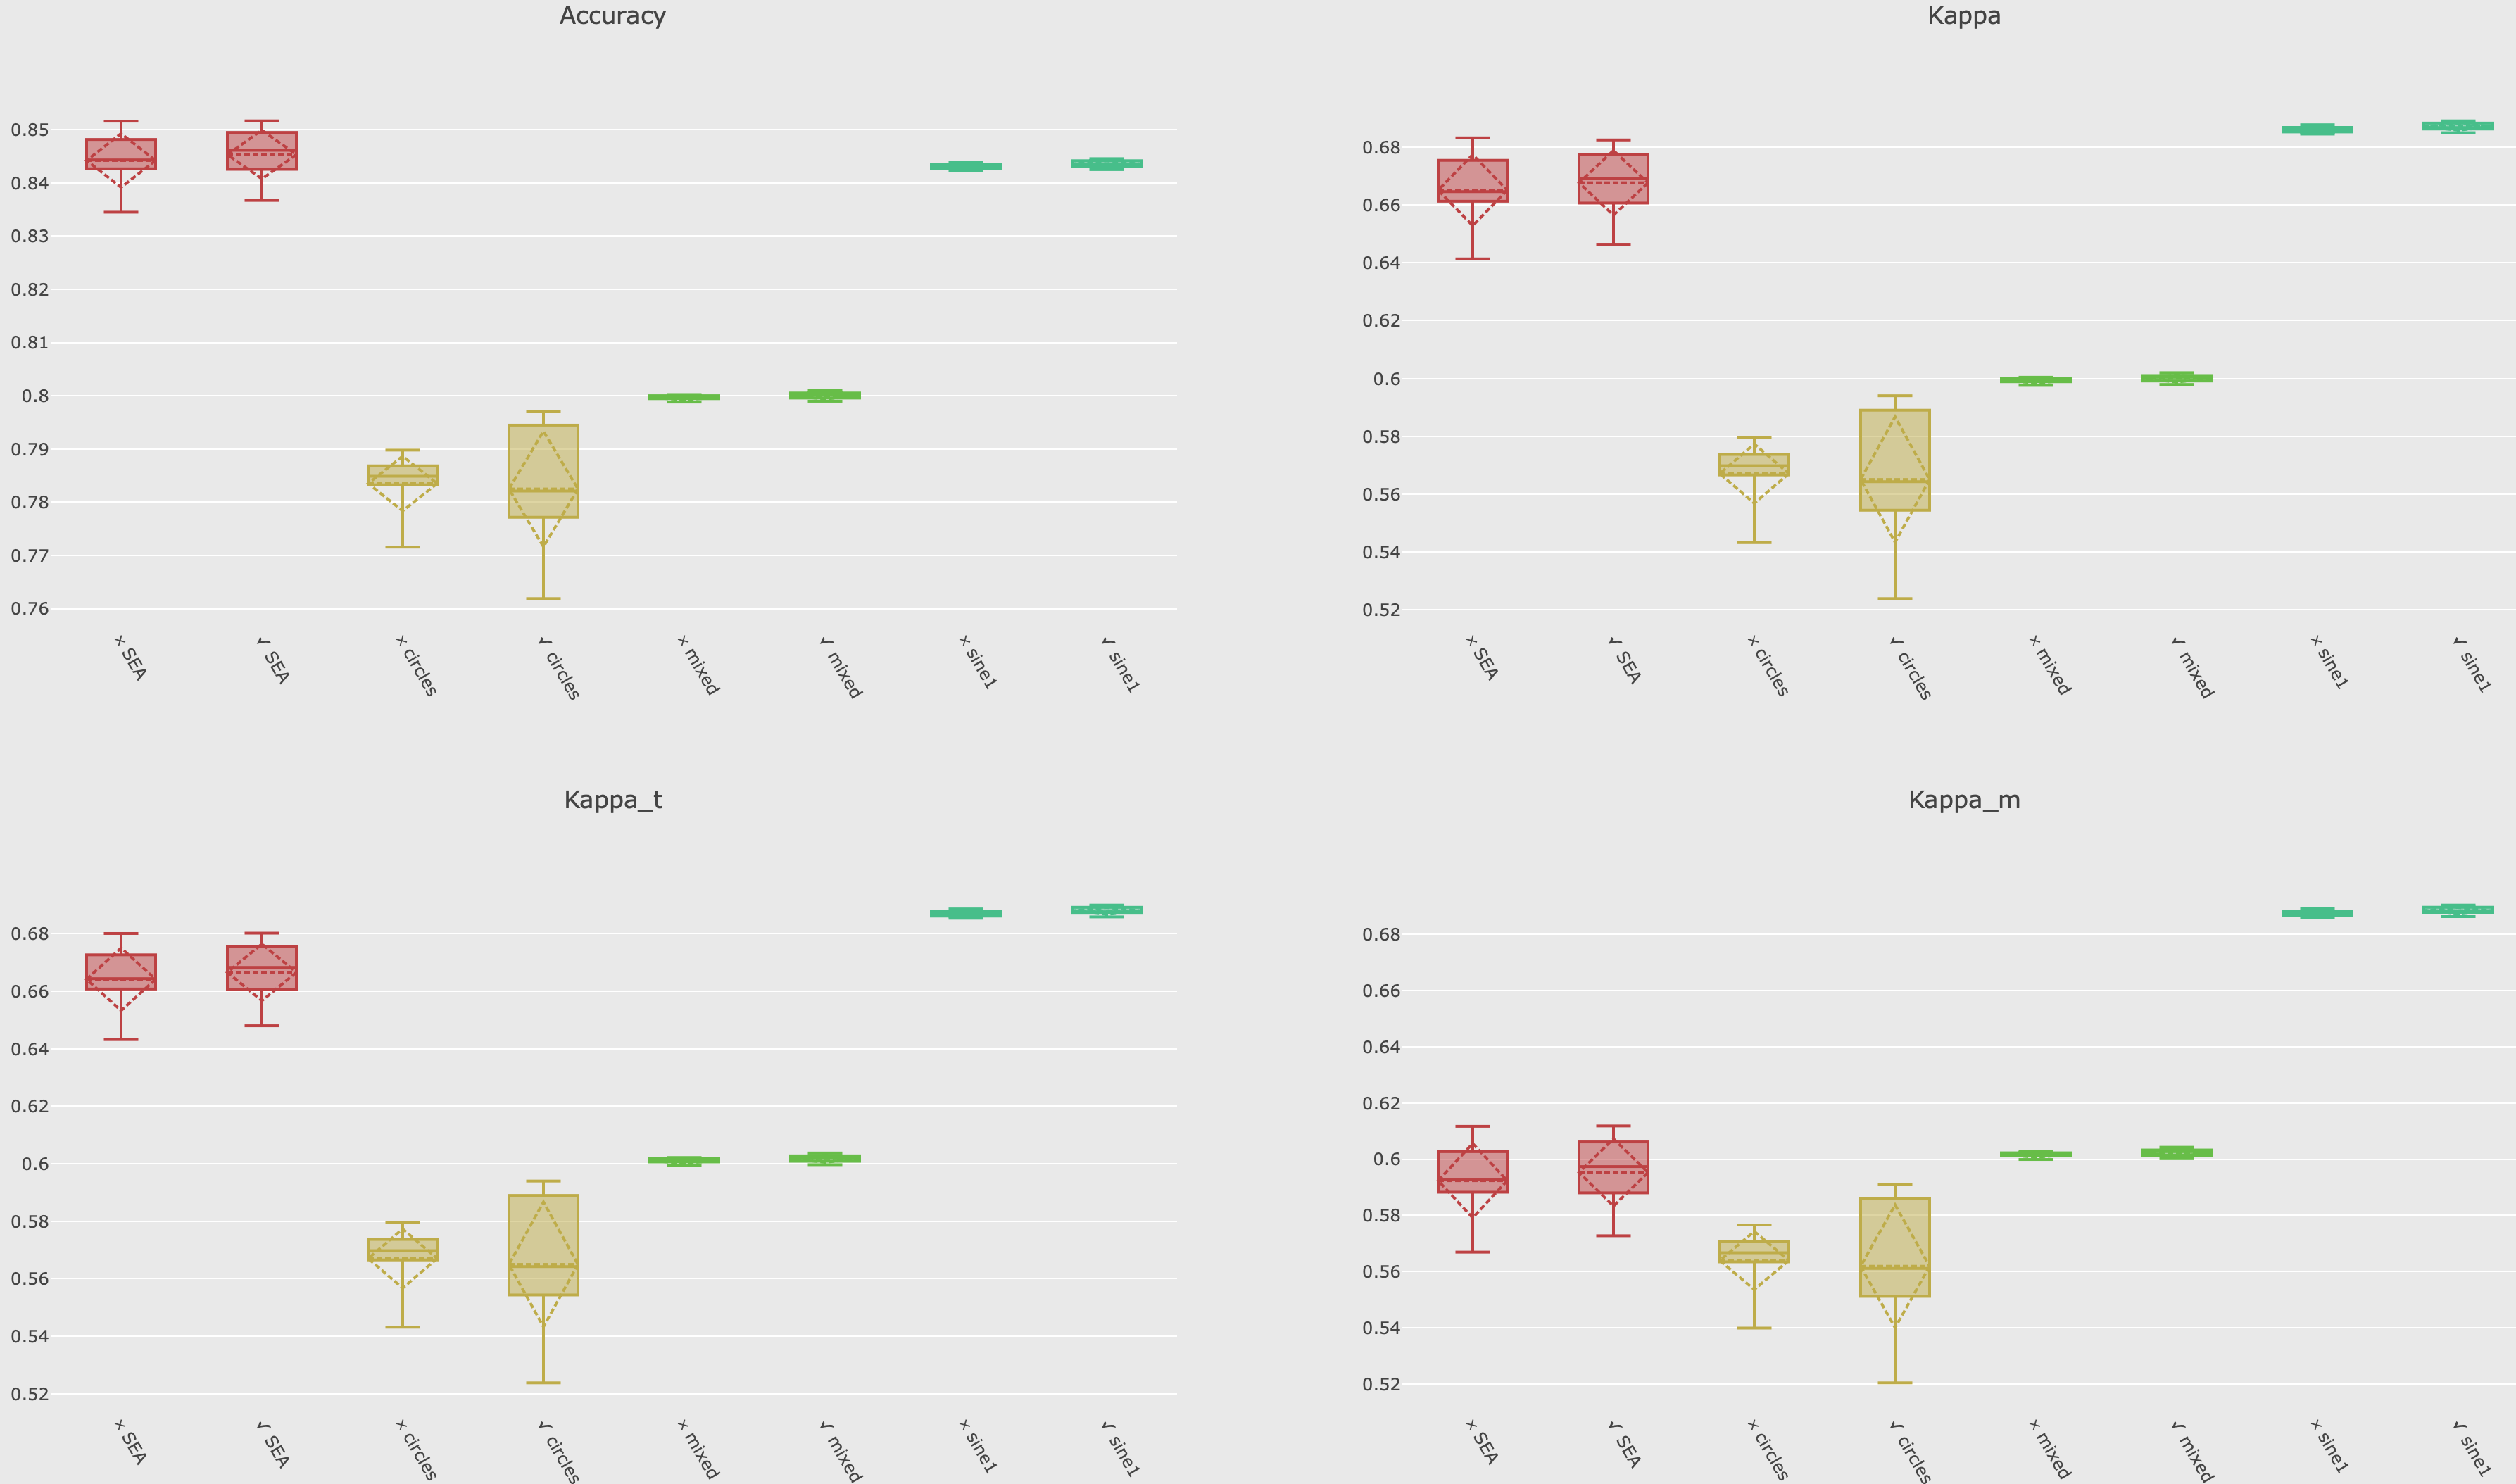
\includegraphics[width=\linewidth]{./images/chapter3/boxplot_params_use_w}
\caption{\label{fig:boxplot_params_use_w}Boxplots showing performance over 4 datasets (using un/weighted probabilities for drift detection)}
\end{figure}

Our modified drift detectors using the probabilities will be called Modified FHDDM/S.
Algorithm \ref{alg:pfhddm} shows the implementation of MFHDDM. No changes were necessary to implement MFHDDM/S with the different boolean, since this is similar to the current version.

\begin{algorithm}[h]
\caption{Modified Fast Hoeffding Drift Detection Method (MFHDDM)\label{alg:pfhddm}}
\Fn{init(window\_size, delta, use\_probability)}{
    (n, $\delta$, p) = (window\_size, delta, use\_probability)\;
    $\epsilon_d = \sqrt{\frac{1}{2n}ln\frac{1}{\delta}}$\;
    reset()\;
}

\Fn{reset()}{
    w=[]\;
    $\mu^m=0$\;
}

\Fn{detect(p)}{
    \If{w.size = n}{
        w.tail.drop()\;
    }
    w.push(p)\;
    \eIf{$w.size < n$}{
        return False\;
    }{
        \eIf{use\_probability}{
            $\mu^t=w.average()$\;
        }{
            $\mu^t=\frac{w.count(True)}{w.size()}$\;
        }
        \If{$\mu^m < \mu^t$}{
            $\mu^m =\mu^t$\;
        }
        $\Delta\mu = \mu^m - \mu^t$\;
        \eIf{$\Delta\mu \ge \epsilon_d$}{
            reset()\;
            \Return True\;
        }{
            \Return False\;
        }
    }
}
\end{algorithm}

%----------------------------------------------------------------------------------------

\section{A toy example}

In this section, we explain how an instance from the stream is processed from beginning to end. The reader should refer to algorithm \ref{alg:pipeline_pseudocode} and figures \ref{fig:sequence_diagram} and \ref{fig:prequential_loop}.

The first step in the algorithm is to pre-train the algorithm so that it can start with a\textbf{n} adequate model of the data. Therefore a parameter is used to dictate the number of instances that the ensemble is trained on before starting the interleaved test-then-train loop.

Next, the interleaved test-then-train loop begins. For this toy example, we use a batch size of one. This batch (or chunk) contains a single instance, which is referred to as $X$, and its true class value is referred to as $y$.

The ensemble is first tasked with predicting the class value, denoted $\hat{y}$, of $X$. In order to do so, the ensemble requires each classifier it contains to assign a probability that $X$ belongs to a class, for each possible value that the class can take. We use binary classification as example, therefore \textbf{$y \in \{0,1\}$}. So in our example, each classifier needs to predict $P(X, y=0)$, and $P(X, y=1)$ given its model of the data. The ensemble then keeps a copy of these predictions and applies a weighting function to the original values. The weighting function, as previously stated, reduces values in $]0,0.5[$ and increases values in $]0.5, 1[$. Finally, the ensemble averages the probabilities for each class class value (again, for binary classification). It continues in the same manner for the weighted probabilities. The ensemble now has four values: $p_0, p_1 = \frac{1}{n}\sum_{i=1}^{n} P_i(X, y=Y)\ \forall\ Y$,  $w_0,w_1=\frac{1}{n}\sum_{i=1}^{n} w(P_i(X, y=Y))\ \forall\ Y$, where $n$ is the number of classifiers in the ensemble, $w(x)$ is the weighting function seen in section \ref{section:new_voting_strategy}, $P_i(X, y=0)$ is the probability that classifier $i$ assigns $X$ to class $0$. $Y$ is the set of possible class values.
The maximum of $p_0$ and $p_1$ determines the class the ensemble predicts for $X$. If $p_0$ is the maximum value, then $\hat{y}=0$, and in the opposite case where $p_1$ is the maximum value then $\hat{y}=1$.

The next step in the interleaved test-then-train loop is dedicated to drift detection. In the case \textbf{where }a drift is detected, a sliding window keeps the previously seen instances for retraining the classifiers. The size of this window is the same as the size of the window used for the training step, therefore it is size three in our example. MFHDDMS is used to detect drifts, when its sliding window it full. The average probability for the winning class, is passed to the drift detector. There are two sliding windows: one short to detect abrupt drifts, and a longer one to detect gradual concept drifts. The sliding window, therefore, keeps track, as discussed in section \ref{section:new_voting_strategy}, of either probabilities or booleans. In the case of the probabilities, the Hoeffding bound is used to detect if the average probability drifts too far from the maximum seen average probability. In the case of the boolean values, a drift is detected, using the Hoeffding bound again, when the classifier in question predicts less often on average according to the "winning" vote.
When a drift is detected, the drift detector's windows are emptied, the classifiers in the ensemble are either all reset or a subset of them are reset. 
If a drift is detected, the sliding window of previously seen instances is then used to retrain all of the classifiers in the ensemble.

If no drift is detected, there is a chance (set by a parameter) that the $y$ value (the real class value of $X$) will be replaced by $\hat y$ (the predicted class value of $X$). This serves as the self-training step, where the parameter would force $X$ to be unlabelled.

The final step in the interleaved test-then-train loop is to train the ensemble on the $<X, y>$ tuple. In order to do so, a hybrid sliding-tumbling window (as seen in section \ref{section:hybrid-windows}) is used within the ensemble to train the classifiers contained within it. In this case, since $<X, y>$ is the first instance seen by the ensemble during the interleaved test-then-train loop (as in this is the first iteration of the prequential evaluation loop) it is added to the hybrid window. This hybrid window has a size equal to the batch size (in this case, one) times the number of classifiers in the ensemble (three). 
Only one classifier in the ensemble is trained on the hybrid window's tuples. In order to do so, an index is kept inside the ensemble. This index points to the classifier to train and is incremented at each $ensemble.train()$ call, and a modulus is applied on the index to keep it within the range of classifiers in the ensemble.
Thus, classifier $c_0$ is selected to train on the hybrid window, containing a single tuple at the moment.

At this point, the first iteration of the interleaved test-then-train loop has terminated, and the framework computes the global metrics required (accuracy, kappa statistics, etc.) as well as over a sliding window of the last 200 instances.

\begin{algorithm}
\caption{Data processing pipeline\label{alg:pipeline_pseudocode}}
\Fn{evaluate\_prequential(ensemble, pretrain\_size, batch\_size, window\_size)}{
    ensemble.train(pretrain\_size)\;
    window = fifo\_queue(size = window\_size)\;
    \While{stream.has\_more\_samples()}{
        X, y = stream.next\_sample(batch\_size)\;
        window.add([X,y])\;

        prediction, probabilities, weighted\_probabilities = ensemble.test(X)\;
        
        drift\_detected = drift\_detection(prediction\ \textbf{or}\ probabilities\ \textbf{or}\ weighted\_probabilities)\;

        \If{random() > ground\_truth\_percentage \textbf{and}\ not\ drift\_detected}{
            replace\_y(y, prediction)\;
        }
        
        \If{drift\_detected}{
            ensemble.reset(window)\;
        }
        
        ensemble.train(X, y)\;
    }
}

\Fn{ensemble.train(X, y)}{
    \tcp{instance variables $clfs$ stores the classifiers in ensemble \& $mod$ stores the current index 
    of the classifier to train}
    ensemble.clfs[ensemble.mod].train(X, y)\;
    ensemble.mod = (ensemble.mod + 1) modulus (length(ensemble.clfs))\;
}

\Fn{ensemble.test(X)}{
    p, w\_p = [], []\;
    \For{$classifier \in ensemble.classifiers$}{
        prob = classifier.predict()\;
        p.add(prob), w\_p.add([weight(prob[0]), weight(prob[1]))\;
    }
    \tcp{map subclassifier probabilities to single probability}
    avg, w\_avg = p.avg(), w\_p.avg()\;
    prediction = class\_of\_max(w\_avg)\;
    \Return prediction, avg, w\_avg\;
}

\Fn{weight(prediction\_probability)}{
    \Return $\frac{1-tanh(3.5-7\times prediction\_probability)}{2}$\;
}

\Fn{drift\_detection(value, use\_probability)}{
    window.push(value)\;
    \If{$window.size > max\_window\_size$}{
        window.tail.drop()\;
        \eIf{use\_probability}{
            $\mu^t=window.average()$\;
        }{
            $\mu^t=\frac{window.count(True)}{window.size()}$\;
        }
        \If{$\mu^m < \mu^t$}{
            $\mu^m =\mu^t$\;
        }
        $\Delta\mu = \mu^m - \mu^t$\;
        \If{$\Delta\mu \ge \epsilon\_d$}{
            \Return True\ \textbf{and} reset();
        }
    }
    \Return False\;
}
\end{algorithm}

\begin{figure}
  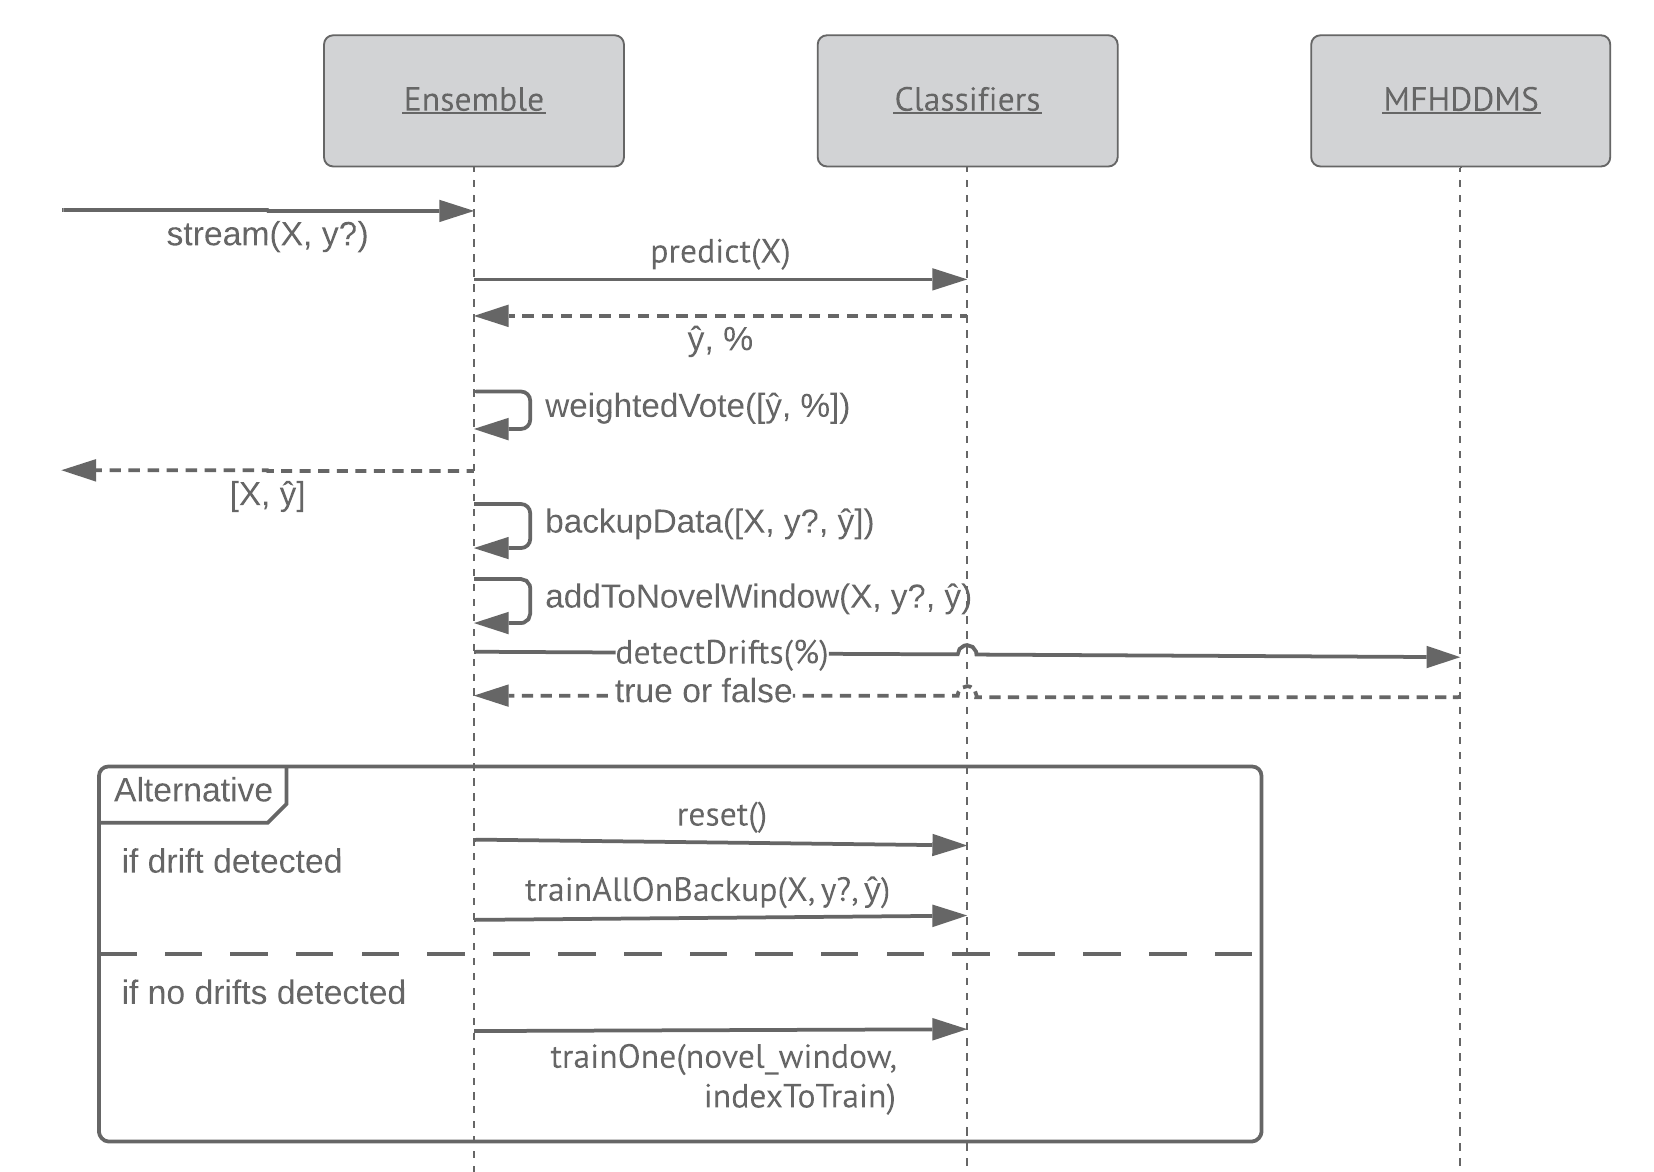
\includegraphics[width=\linewidth]{./images/chapter3/sequence_diagram}
\caption{\label{fig:sequence_diagram}Simplified Sequence Diagram illustrating algorithm \ref{alg:pipeline_pseudocode}}
\end{figure}

%----------------------------------------------------------------------------------------

\section{Conclusion}
In this chapter, we have introduced the components of our LESS-TWE methodology. The first contribution was to propose a new weighting function for our ensemble classifier. The second was a novel windowing technique for classifiers within an ensemble that delays their training. The third was the non-selective self-training on a portion of the training data (for which the label was ignored). The fourth and final contribution was to extend FHDDM/S to operate without any knowledge of the ground truth. We described the components of our methodology and their algorithms, and illustrated the framework by means of a toy example.Next, we explain our experimental evaluation.